\documentclass[a4paper,12pt]{article}
\usepackage[T1]{fontenc}
\usepackage{graphicx}
\usepackage{lipsum}

\begin{document}

\section{Float placement}

\lipsum[2-3]

\par\noindent
\textbf{MARKER A: first portrait declared here.}
\par

\begin{figure}[h]
    \centering
    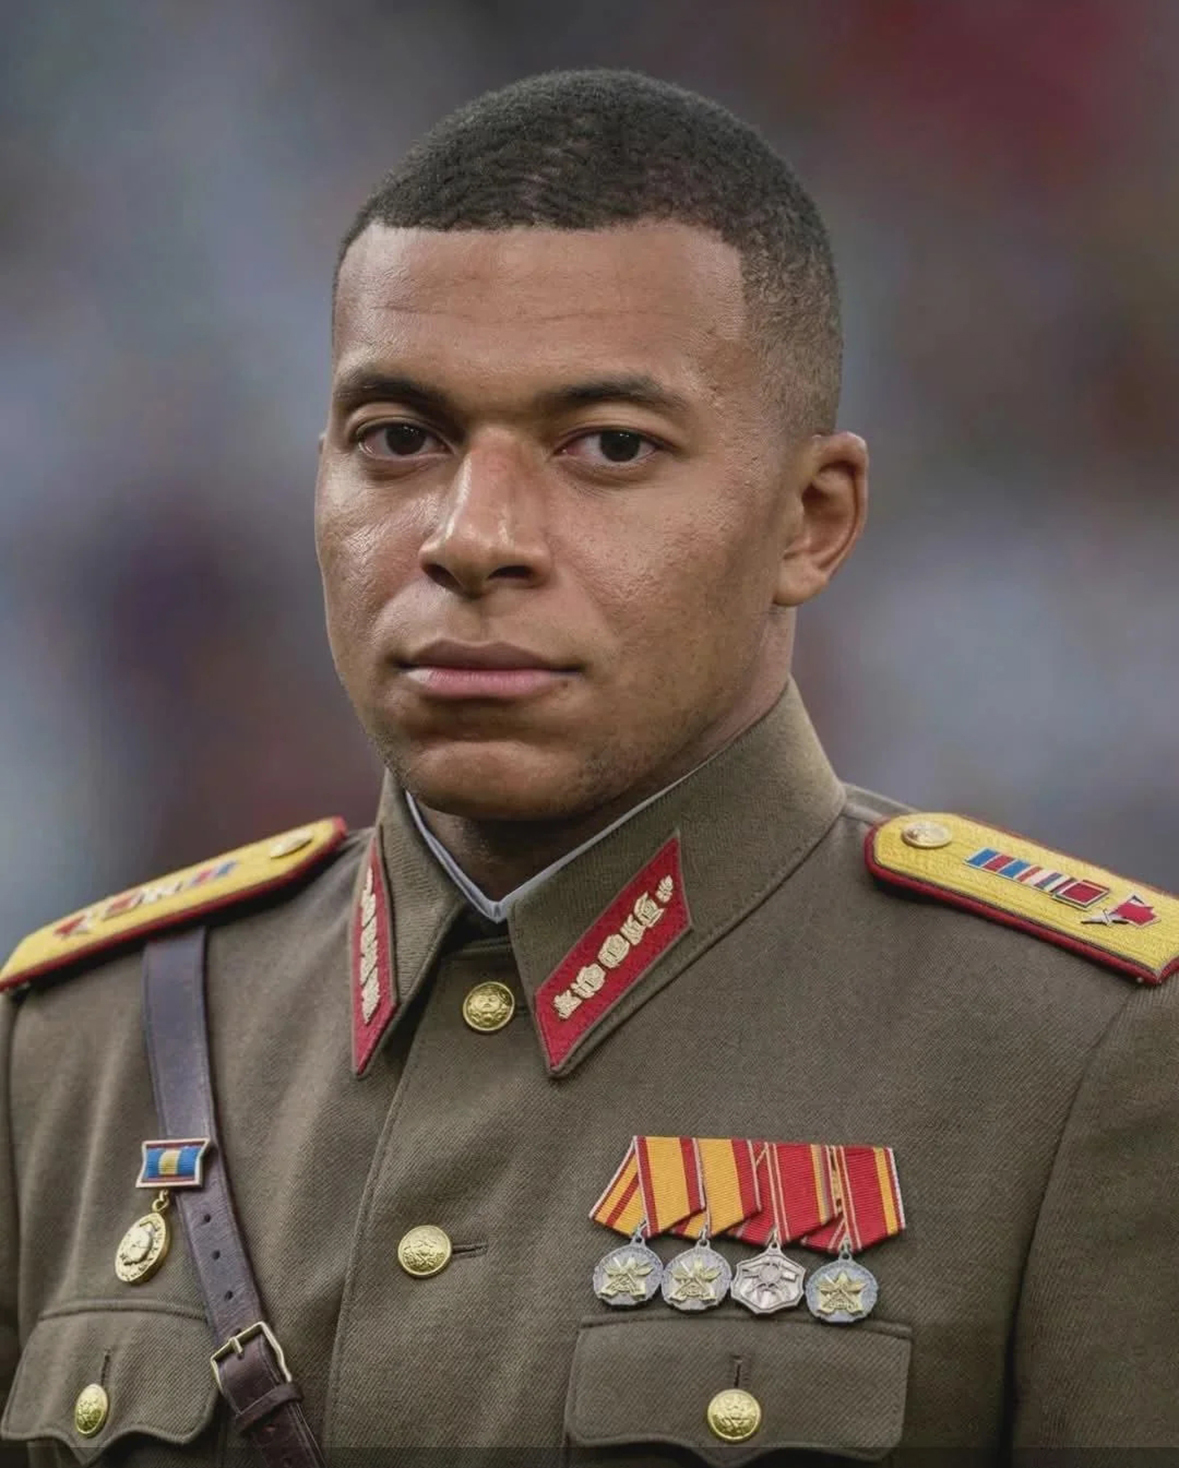
\includegraphics[height=4.2cm]{../../pix/mbappe.jpg}
    \caption{Portrait A: placement h.}
    \label{fig:placement-h}
\end{figure}

\lipsum[5-6]

\par\noindent
\textbf{MARKER B: second portrait declared here.}
\par

\begin{figure}[t]
    \centering
    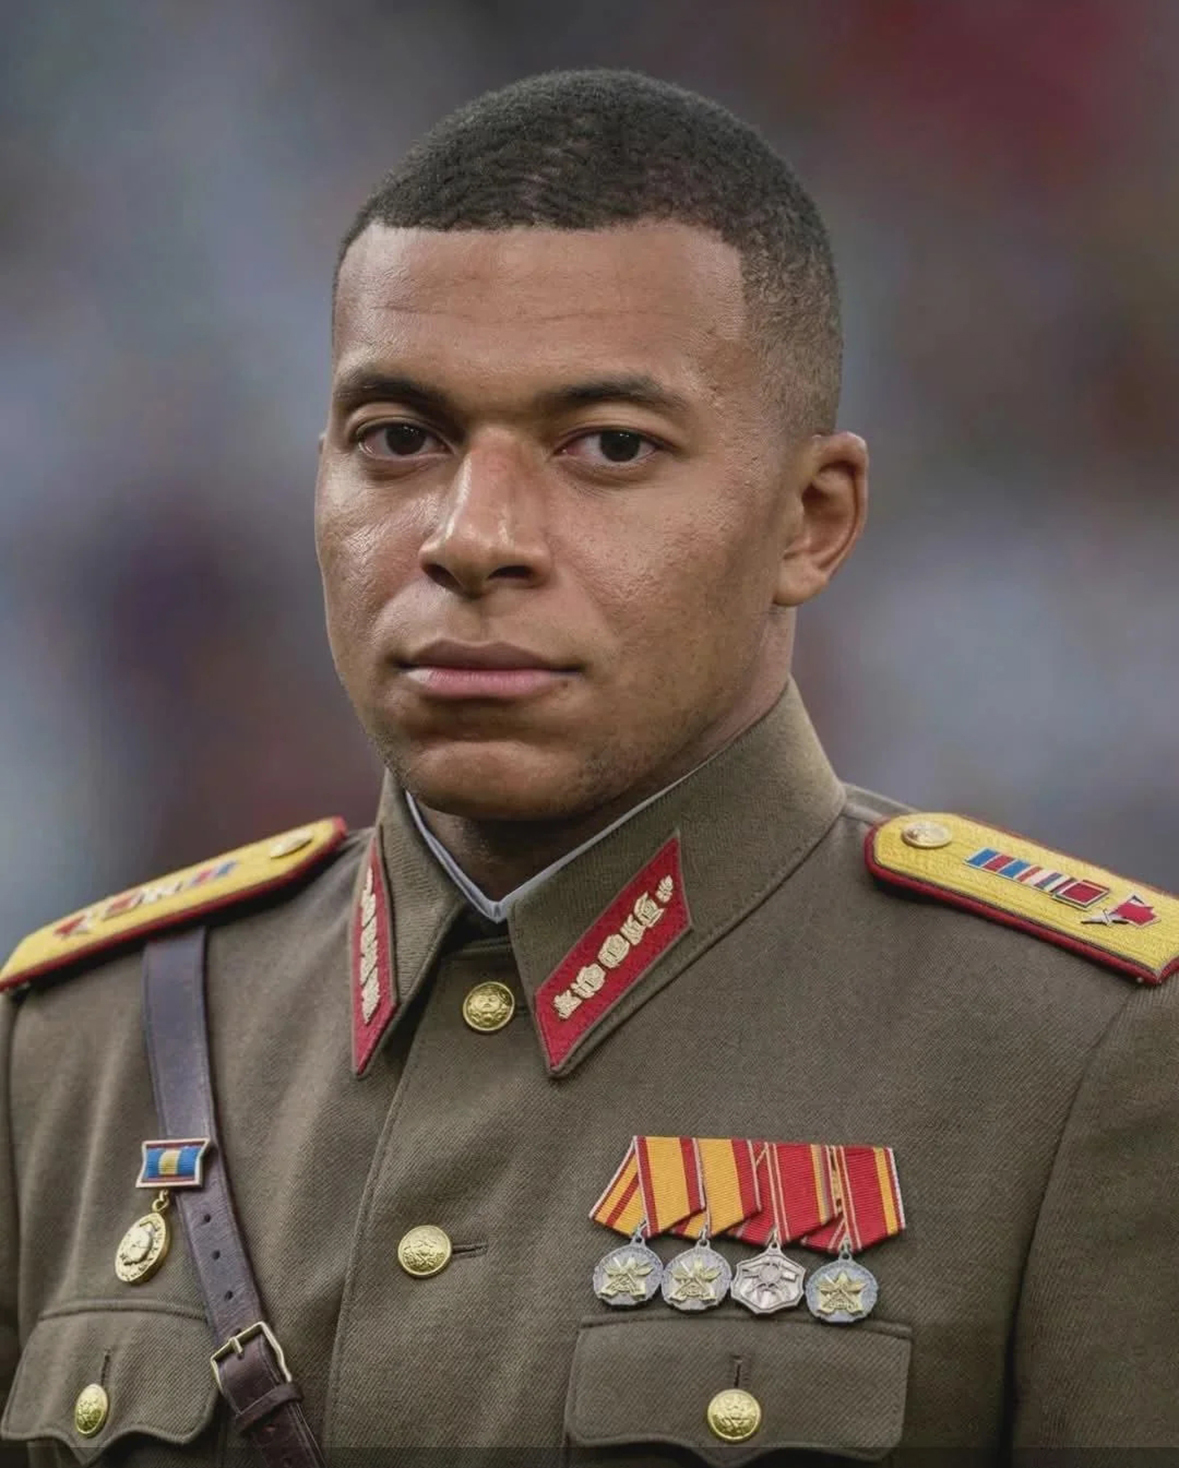
\includegraphics[height=4.2cm]{../../pix/mbappe.jpg}
    \caption{Portrait B: placement t.}
    \label{fig:placement-t}
\end{figure}

\lipsum[8-9]

\par\noindent
\textbf{MARKER C: third portrait declared here.}
\par

\begin{figure}[b]
    \centering
    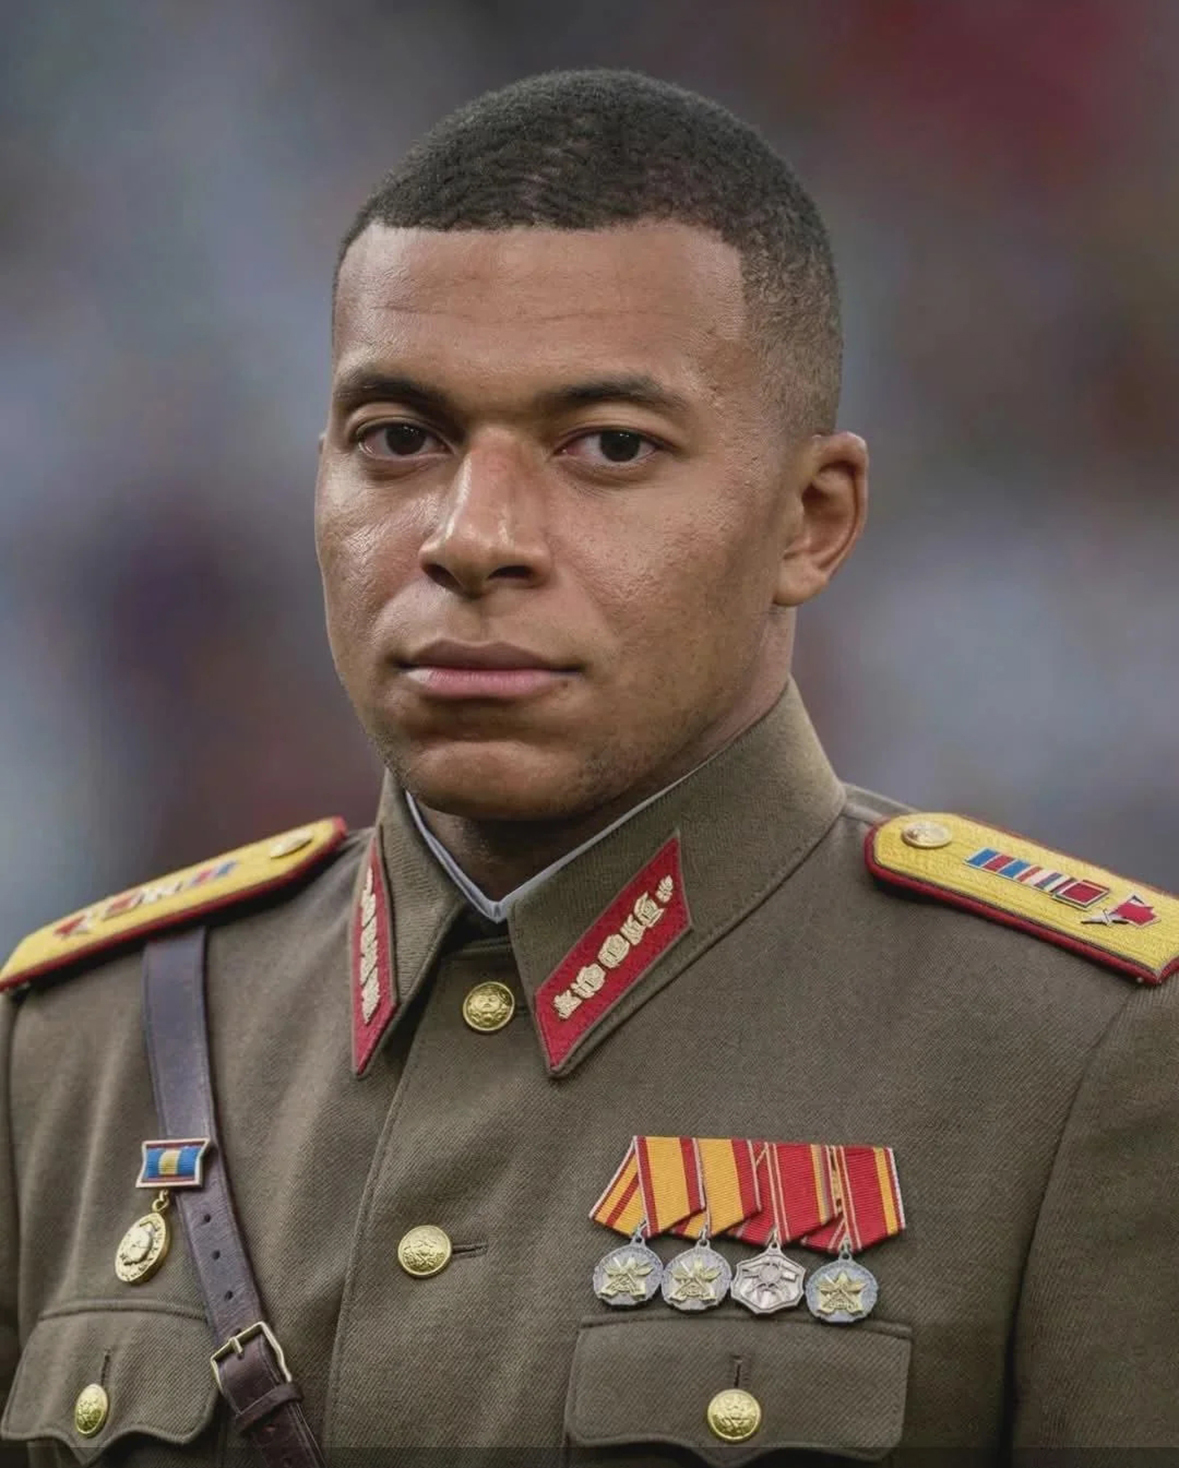
\includegraphics[height=4.2cm]{../../pix/mbappe.jpg}
    \caption{Portrait C: placement b.}
    \label{fig:placement-b}
\end{figure}

\lipsum[11-12]

\par\noindent
\textbf{MARKER D: fourth portrait declared here.}
\par

\begin{figure}[p]
    \centering
    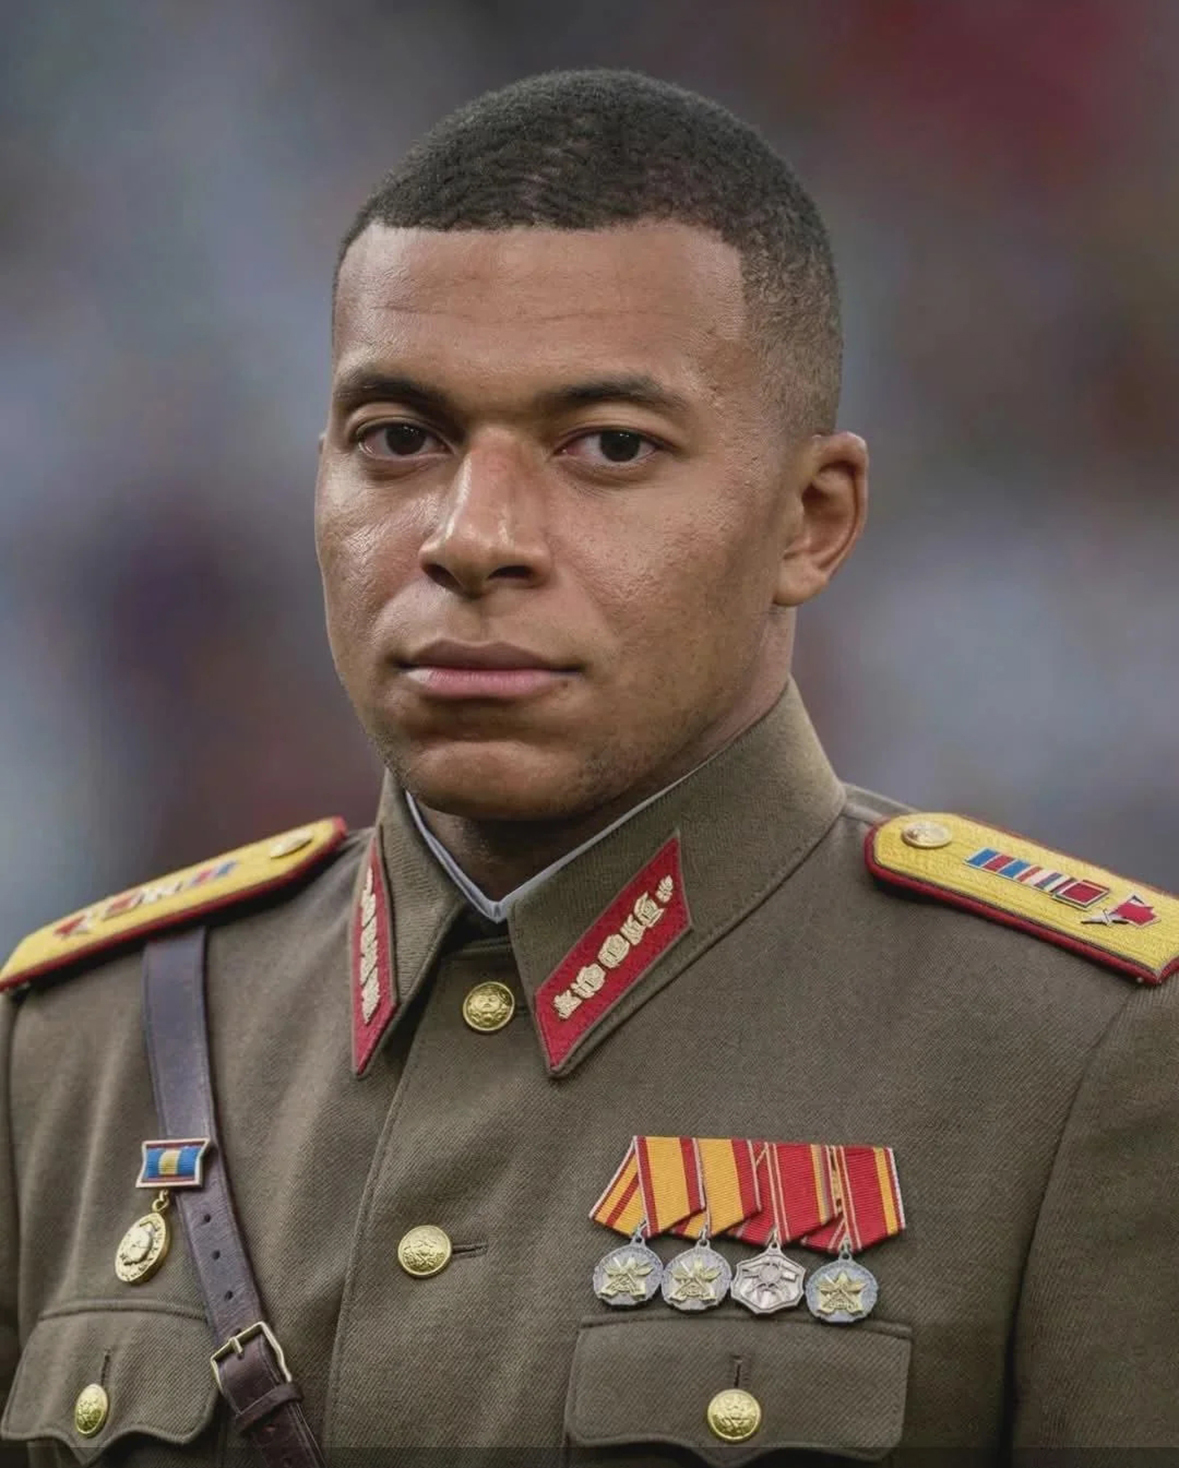
\includegraphics[height=4.2cm]{../../pix/mbappe.jpg}
    \caption{Portrait D: placement p.}
    \label{fig:placement-p}
\end{figure}

\lipsum[14-15]

\par\noindent
\textbf{MARKER E: fifth portrait declared here.}
\par

\begin{figure}[htbp]
    \centering
    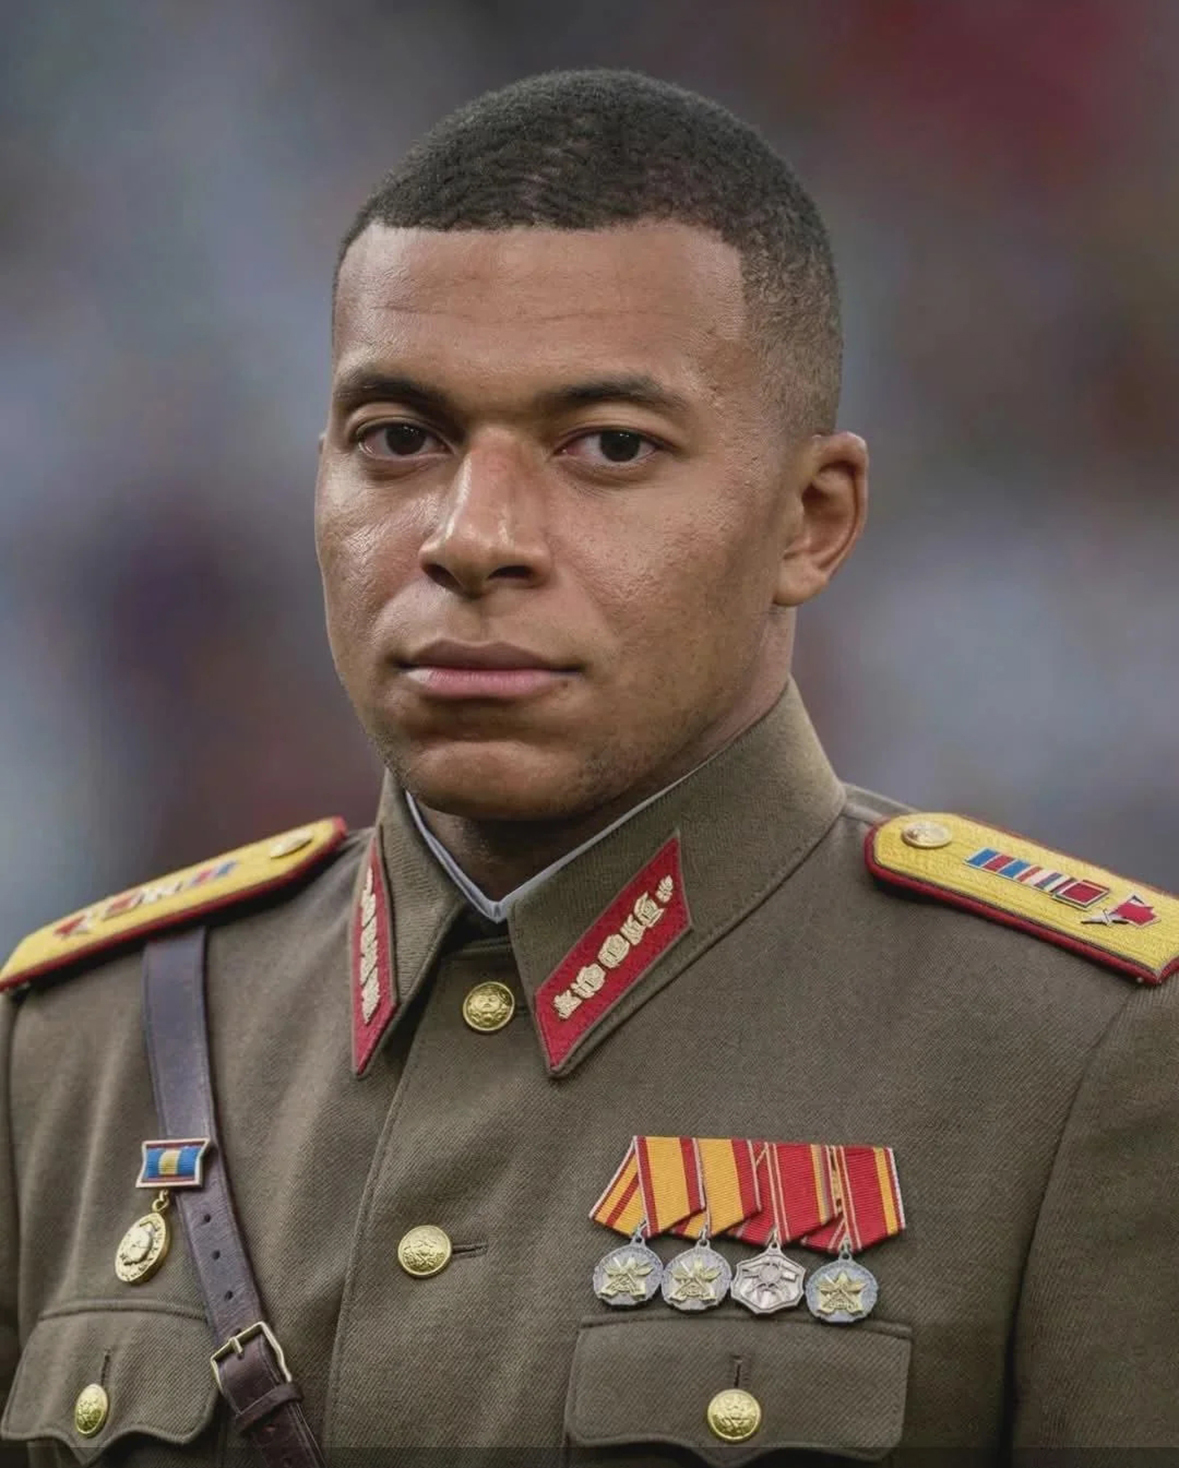
\includegraphics[height=4.2cm]{../../pix/mbappe.jpg}
    \caption{Portrait E: placements h, t, b, p.}
    \label{fig:placement-all}
\end{figure}

\lipsum[17-18]

Compare Figures~\ref{fig:placement-h}--\ref{fig:placement-all}
with their markers in the text.

\clearpage
\end{document}